\documentclass[12pt,a4paper]{article}
\usepackage{ctex}
\usepackage{amsmath}
\usepackage{amsfonts}
\usepackage{amssymb}
\usepackage{makeidx}
\usepackage{graphicx}
\usepackage{xcolor}
\usepackage{listings}
\usepackage[colorlinks,linkcolor=black,urlcolor=black]{hyperref}
\usepackage[left=2.5cm, right=2.5cm, top=2.54cm, bottom=2.54cm]{geometry}
\lstset{numbers=left,frame=single,
	breaklines,
	tabsize=2,
	extendedchars=ture}
\title{\textbf{\CJKfamily{hei}{\huge 集成电路设计实验报告}}}
\author{\textbf{himingway}}
\date{2015年12月1日}
\begin{document}
	\maketitle
	\tableofcontents
	\newpage
	\section{实验目的}
	通过交通灯的设计仿真和综合,体会复杂时序的实现方法,学会用框图表示程序的设计思路,掌握中小规模集成电路的设计方法及仿真技巧。
	\section{设计要求}
	
	设计一个十字路口交通信号灯的控制电路。要求红、绿灯按一定的规律亮和灭,并在亮灯期间进行倒计时,且将运行时间用数码管显示出来。绿灯亮时,为该车道允许通信信号,红灯亮时,为该车道禁止通信信号。要求主干道每次通行时间为Tx秒,支干道每次通行时间为Ty秒。每次变换运行车道前绿灯闪烁,持续时间为5s,即车道要由X转换为Y时,X在通行时间只剩下5秒钟时,绿灯闪烁显示,Y仍为红灯。
	\section{摘要}
	本十字路口交通信号灯的控制电路课程设计给出了流程图、模块设计原理图、时序逻辑设计状态机和其他重要的模块设计(分频器和数码管显示模块),给出了各个模块的verilog代码和编译结果,并用modelsim仿真出波形,对波形做了进一步的分析。并给出了真实FPGA测试的结果,测试结果的正常标志着本设计的圆满完成。最后写下来自己在设计中遇到的一点点小问题,留给以后学习思考解决。	
	\section{项目链接}
		\textbf{Github:}\url{https://github.com/himingway/traffic_light}
		
		\textbf{网站:}\url{http://www.turnright.xyz/archives/1241.html}
		
	\section{设计方案}
		\subsection{设计思路}
		整个设计分为三个部分。第一个部分是顶层模块,将各个模块封装起来。第二个部分是控制模块,用来控制“交通灯”的亮灭。第三个部分是“倒计时产生”模块,用来产生倒计时数。第四个部分是“数码管显示"模块,包括数字取模、BCD编码和数码管段选与位选这三个部分。
		
		其中控制模块、和“倒计时产生”采用周期为10Hz的时钟作为输入时钟,“数码管显示”模块采用较高的时钟频率输入。
		
		\subsection{设计流程图}
		\begin{center}
			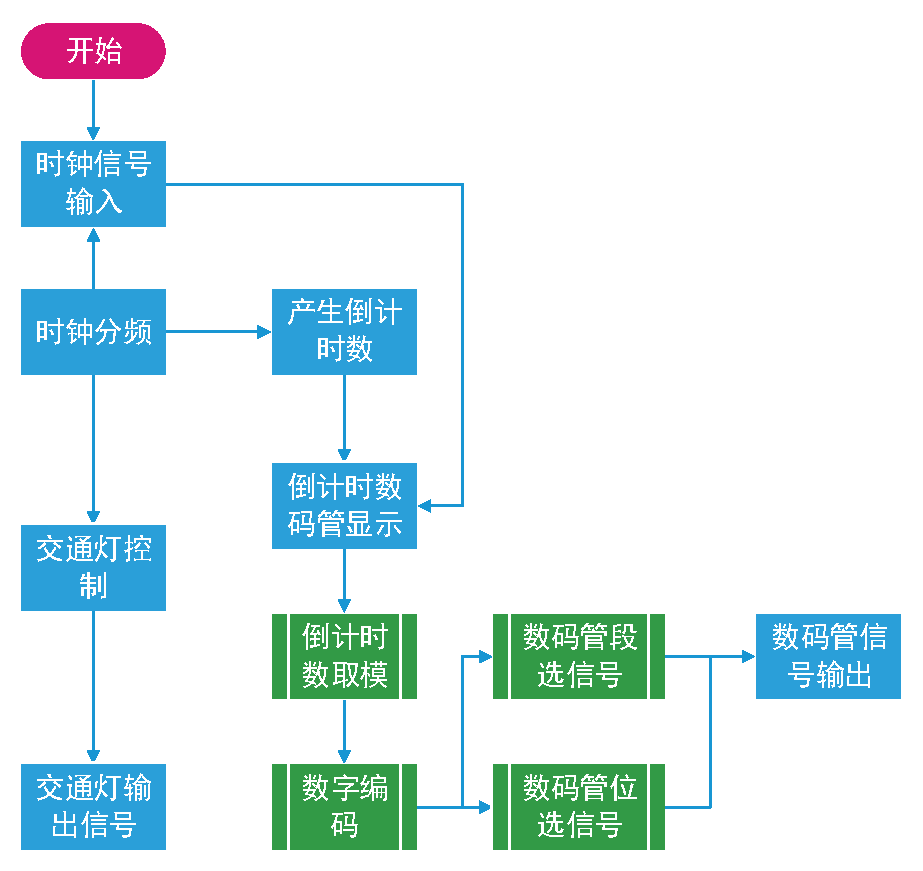
\includegraphics[width=14cm]{pic/lct.eps}
		\end{center}
	\section{模块设计}
	\subsection{顶层模块}
	\begin{center}
		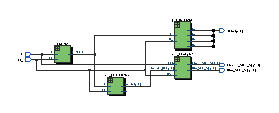
\includegraphics[width=16cm]{pic/pdf/top.eps}
	\end{center}
		\subsubsection{顶层模块功能}
			\begin{itemize}
				\item clock 模块:产生周期为100ms的时钟。
				\item light\_control 模块:产生控制“交通灯”亮灭的信号。
				\item num\_generate 模块:产生“倒计时数字”信号。
				\item num\_display 模块:控制数码管显示“倒计时数字”
			\end{itemize}
		\subsubsection{顶层模块端口}
			\begin{itemize}
				\item clk:时钟信号输入。
				\item rst\_n:异步复位信号输入。
				\item ledout:“交通灯”亮灭的信号输出。
				\item Column\_Scan\_Sig:数码管位选信号输出。
				\item Row\_Scan\_Sig:数码管段选信号输出。
			\end{itemize}
		\subsection{num\_display 模块}
		\begin{center}
				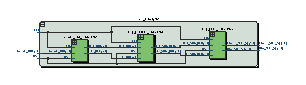
\includegraphics[width=16cm]{pic/pdf/numdisplay.eps}
		\end{center}
		\begin{itemize}
			\item number\_mod\_module:数字取模模块。
			\item smg\_encoder\_module:数码管编码模块。
			\item smg\_scan\_module:数码管扫描模块(用于位选和段选)
		\end{itemize}
		
			\emph{其中"column\_scan\_module"用于位选,"raw\_scan\_module"用于位选}
			
			\begin{center}
				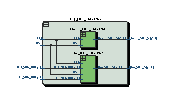
\includegraphics[width=15cm]{pic/pdf/smgscan.eps}
			\end{center}
	\section{时序逻辑设计}
	\subsection{“交通信号灯”控制时序逻辑设计}
		\subsubsection{module light\_control 状态图}
		\begin{center}
		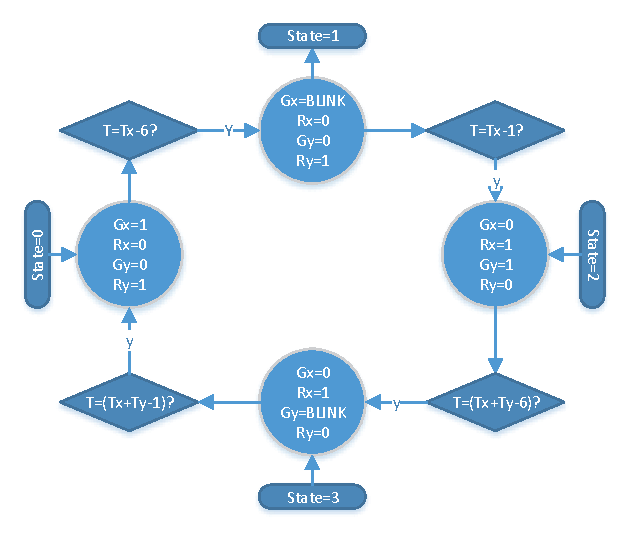
\includegraphics[width=15cm]{pic/statemachine.eps}
		\end{center}
		
	\subsubsection{图例}	
	\begin{center}
			\begin{tabular}{|c|c|}
			\hline Gx & X车道绿灯 \\ 
			\hline Rx & X车道红灯 \\ 
			\hline Gy & Y车道绿灯 \\ 
			\hline Ry & Y车道红灯 \\ 
			\hline BLINK & 闪烁 \\ 
			\hline Tx & X车道通行时间 \\ 
			\hline Ty & Y车道通行时间 \\ 
			\hline 
		\end{tabular}
	\end{center} 
	
	\subsubsection{module light\_control 状态图解释}		
	开始时,X车道绿灯亮红灯灭(state=0),Y车道绿灯灭,红灯亮,计数器从0开始计数,当计数器计数了(Tx-6)个数时,进入X车道绿灯闪烁状态(state=1)。这时,计数器接着计数,当计数器计数了(Tx-1)个数时,X车道绿灯停止闪烁,变为熄灭状态,红灯开始亮;Y车道绿灯亮,红灯灭。即进入(state=3)状态。(state=3)状态和(state=4)状态与(state=0)、(state=1)状态类似,经过一个周期(T=Tx+Ty)时长的循环,状态机重新回到初始的状态。
	
	\subsection{“倒计时数字”模块时序逻辑图}
		\subsubsection{num\_generate 状态图}
		\begin{center}
		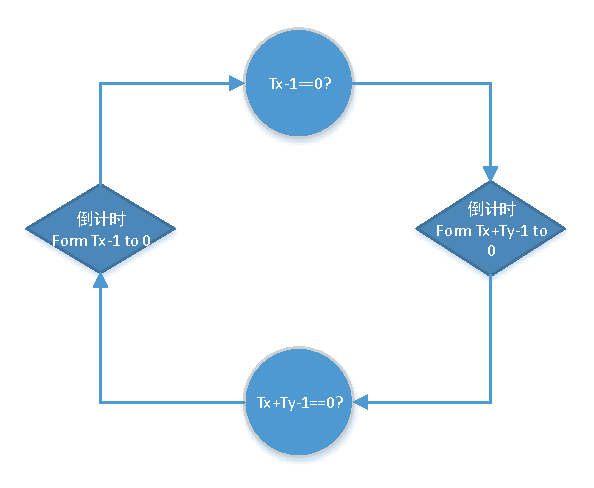
\includegraphics[width=13cm]{pic/num.eps}
		\end{center}
	\subsubsection{num\_generate 状态图解释}
	这是一个倒计时数产生模块,功能是产生“交通灯”所需要的倒计时数,以便于将倒计时数信号输入到数码管显示模块中。该模块时序功能很简单。当X车道通行时,计数器从(Tx-1)计数到0;当Y车道通行时,计数器从(Ty-1)计数到0。
	
	\section{其他模块的设计}
	\subsection{分频器设计}
	\subsubsection{分频器介绍}
	分频器是指使输出信号频率为输入信号频率整数分之一的电子电路。在许多电子设备中如电子钟、频率合成器等,需要各种不同频率的信号协同工作,常用的方法是以稳定度高的晶体振荡器为主振源,通过变换得到所需要的各种频率成分,分频器是一种主要变换手段。
	\subsubsection{分频器设计实现}
	测试所用的硬件时钟输入频率是50MHz,也就是晶振1s震荡50M次。本次设计要得到10Hz的时钟信号,需要用分频器对输入时钟进行分频。
	
	下面对时钟频率进行计算:
	
{\small 	
	\textit{1.FPGA的时钟频率是 50MHz = 50\_000\_000Hz}
	
	\textit{2.要得到10Hz的时钟,计数器数到 50\_000\_000 / 10 = 5\_000\_000,输出时钟为一个周期。}
	
	\textit{3.输出时钟的波形跳变(0变为1或者1变为0)时间为 5\_000\_000 / 2 = 2\_500\_000。}
	
	\textit{4.由于计数器从0开始计数,相应的次数应该减去1。即5\_000\_000 -1 = 4\_999\_999,2\_500\_000 -1 = 2\_499\_999。}}
	\subsection{数码管显示模块}
	\subsubsection{数码管驱动电路}
		\begin{center}
			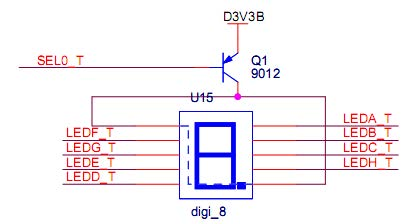
\includegraphics{pic/smg} 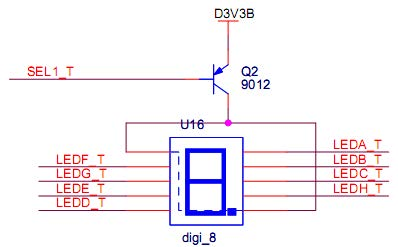
\includegraphics{pic/smg2}
		\end{center}
		
	数码管是共阳,而是用PNP管来反响驱动并且控制列扫描(SEL0\_T和SEL1\_T)。而且所有的数码管的“段选信号”(LEDA .. LEDH)都共用同样的引脚。结论来说,数码管都信号都是“低电平有效”。
	\subsubsection{数字取模模块}
	“number\_mod\_module.v”的设计是利用数学运算符“\%”和“/”分别取得十位和个位。因为是十位取位的关系,所以最大的输入数是00\~99而已。
	
	\begin{center}
	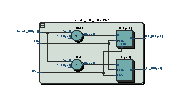
\includegraphics[width=15cm]{pic/pdf/nummod.eps}
	\end{center}
	\subsubsection{数码管段选和位选模块}
	\begin{center}
	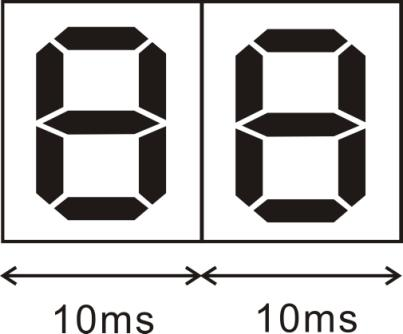
\includegraphics{pic/smg1}
	\end{center}

	因为要求是两个数码管资源,假设各个数码管点亮时间是10ms,两个数码管所占用的时间自然是20ms。换句话说,就是完成一次扫描占用20ms的周期时间。column\_scan\_module.v是负责“列扫描”,亦即每隔10ms就使能(点亮)不同的数码管。row\_scan\_module.v主要是每隔10ms,输出不同的数码管码。
	\section{verilog 代码}
	\subsection{traffic\_light.v}
	这是本设计的顶层模块,包含了所有模块的全部功能。
	
	该模块设置了两个参数,Tx和Ty,当修改X车道和Y车道的通行时间时,仅仅需要改动参数大小即可,无需改变整个代码。这是本设计的优点。
	\begin{lstlisting}[language=Verilog]
module traffic_light (
	input clk,    // Clock
	input rst_n,  // Asynchronous reset active low
	output [7:0]Row_Scan_Sig, //数码管段选
	output[1:0]Column_Scan_Sig, //数码管位选
	output [3:0]ledout //灯控制输出
);

parameter Tx=30; //X车道通行时间
parameter Ty=15; //Y车道通行时间

wire clk100ms;
wire [7:0] Numout;
clock U1 //时钟模块
(
	.clk(clk),
	.rst_n(rst_n),
	.clk100ms(clk100ms)
	);

light_control #(Tx,Ty) U2 //交通灯控制模块
(
	.clk(clk100ms),
	.rst_n(rst_n),
	.Gx(ledout[0]),
	.Rx(ledout[1]),
	.Gy(ledout[2]),
	.Ry(ledout[3])
	);

num_generate #(Tx,Ty) U3 //倒计时数参数模块
(
	.clk(clk100ms),
	.rst_n(rst_n),
	.Numout(Numout)
	);

num_display U4 //倒计时数显示模块
(
	.CLK(clk),
	.RSTn(rst_n),
	.Number_Data(Numout),
	.Row_Scan_Sig(Row_Scan_Sig),
	.Column_Scan_Sig(Column_Scan_Sig)
	);
endmodule
	\end{lstlisting}
	\subsection{clock.v}
	时钟分频模块,用来产生100ms的周期的时钟。
	
	至于为啥要用100ms的时钟,这里有两个原因。第一个原因是绿灯闪烁周期设为1s,从亮到灭或者从灭到亮分别要用500ms,虽然产生1s周期的时钟更方便些,但是1s周期的时钟无法分成比1s还要小的时钟周期单位,也就是说分频容易倍频难。第二个原因是便于仿真,仿真时,只要输入几百个时钟周期就能完成一个周期的“红绿灯”闪烁功能。
	\begin{lstlisting}[language=Verilog]
/*This module is used to generate the 100ms clock*/
module clock (
	input clk,    // Clock
	input rst_n, // Asynchronous reset active low
	output clk100ms //100ms周期的时钟输出
);
reg [23:0] cnt100ms;
reg rclk100ms;
//the clock of the FPGA is 50MHz=50_000_000HZ
//generate 100ms clock
always @(posedge clk or negedge rst_n) begin : proc_cnt100ms
	if(~rst_n) begin
		cnt100ms <= 0;
		rclk100ms <=0;
	end else begin
		if(cnt100ms == 24'd2_499_999) begin 
			cnt100ms <= 24'd0;
			rclk100ms <= ~rclk100ms;//一个周期计数器计数2_499_999次
		end
		else
			cnt100ms <= cnt100ms + 1'd1;
	end
end
assign clk100ms = rclk100ms;
endmodule	
	\end{lstlisting}
	\subsection{light\_control.v}
	交通灯控制模块,用来产生控制交通灯亮灭的信号。状态图详见\textbf{6.1.1}.
	\begin{lstlisting}[language=Verilog]
module light_control (
	input clk,    // Clock 输入时钟周期为100ms
	input rst_n,  // Asynchronous reset active low
	output Gx,Rx,Gy,Ry 
	/*信号输出,其中Gx为X车道绿灯,Rx为x车道红灯,Gy为x车道红灯,Ry为x车道红灯*/
);

reg rGx;
reg rGy;
reg rRx;
reg rRy;
reg [1:0] state;
reg [23:0] cnt;

parameter Tx =30; //X车道通行时间
parameter Ty = 15; //Y车道通行时间

/*计数器,从(Tx+Ty)*10-1开始倒计数,计数到0然后重新开始计数,在输入时钟周期为100ms的条件下,每一个计数周期用时为(Tx+Ty)秒*/
always @(posedge clk or negedge rst_n) begin : proc_cnt
	if(~rst_n) begin
		cnt <= 0;
	end else begin
		if (cnt == (Tx+Ty)*10-1)
			cnt <= 0;
		else
			cnt <= 1'd1+cnt;
	end
end

\*交通灯控制模块状态机,原理解释详见6.1.3*\
always @(posedge clk or negedge rst_n) begin : proc_light_control
	if(~rst_n) begin
		state <= 2'd0;
		rGx <= 1'd0;
		rGy <= 1'd0;
		rRx <=1'd0;
		rRy <= 1'd0;
	end else begin
		case (state)
			2'd0:begin \\X车道通行,开始倒计时
				if(cnt == Tx * 10 - 51) begin
					state <= 2'd1;
					rGx <= 1'b0;
				end
				else
					rGx <= 1'b1;
					rRy <= 1'b1;
					rRx <= 1'b0;
					rGy <= 1'b0;
			end
			2'd1:begin \\X车道绿灯闪烁
				if(cnt == Tx*10 -1) begin
					state <= 2'd2;
					rGx <= 1'b0;
				end
				else if(cnt == Tx*10 - 6) begin 
					rGx <= 1'b1;
				end
				else if(cnt == Tx*10 - 11) begin 
					rGx <= 1'b0;
					end
				else if(cnt == Tx*10 - 16) begin 
					rGx <= 1'b1;
					end
				else if(cnt == Tx*10 - 21) begin 
					rGx <= 1'b0;
					end
				else if(cnt == Tx*10 - 26) begin 
					rGx <= 1'b1;
					end
				else if(cnt == Tx*10 - 31) begin 
					rGx <= 1'b0;
					end
				else if(cnt == Tx*10 - 36) begin 
					rGx <= 1'b1;
					end
				else if(cnt == Tx*10 - 41) begin 
					rGx <= 1'b0;
					end
				else if(cnt == Tx*10- 46) begin 
					rGx <= 1'b1;
					end
			end
			2'd2:begin \\Y车道通行,开始倒计时
				if(cnt == (Tx+Ty)*10-51) begin 
					state <= 2'd3;
					rGy <= 1'b0;
				end
				else begin
					rRy <=1'b0;
					rGy <= 1'b1;
					rRx <= 1'b1;
				end
			end
			2'd3:begin \\Y车道绿灯闪烁 
				if(cnt == (Tx+Ty)*10-1) begin
					rGy <= 1'b0;
					state <= 2'd0;
				end
				else if(cnt == (Tx+Ty)*10-6) begin 
					rGy <= 1'b1;
				end
				else if(cnt == (Tx+Ty)*10-11) begin 
					rGy<= 1'b0;
					end
				else if(cnt == (Tx+Ty)*10-16) begin 
					rGy <= 1'b1;
					end
				else if(cnt == (Tx+Ty)*10-21) begin 
					rGy <= 1'b0;
					end		
				if(cnt == (Tx+Ty)*10-26) begin
					rGy <= 1'b1;
				end
				else if(cnt == (Tx+Ty)*10-31) begin 
					rGy <= 1'b0;
				end
				else if(cnt == (Tx+Ty)*10-36) begin 
					rGy<= 1'b1;
					end
				else if(cnt == (Tx+Ty)*10-41) begin 
					rGy <= 1'b0;
					end
				else if(cnt == (Tx+Ty)*10-46) begin 
					rGy <= 1'b1;
					end
			end
			default : state <= 2'd0;
		endcase
	end
end

assign Gx = rGx;
assign Gy = rGy;
assign Rx = rRx;
assign Ry = rRy;
endmodule
	\end{lstlisting}
	\subsection{num\_generate}
	数字产生模块,状态图如6.2.1所示。但是这里没有用状态机,用了类似计算机编程语言的顺序写法,效果和状态机完全一致,实现的功能电路也一致,这也本程序的一个尝试。
	\begin{lstlisting}[language=Verilog]
module num_generate (
	input clk,    // Clock
	input rst_n, // Asynchronous reset active low
	output [7:0]Numout, //倒计时数字输出
	);

parameter Tx =30;
parameter Ty = 15;

reg [7:0] rNumout = Tx-1;
reg [8:0]cnt1;
reg clk1;
reg flag;

always @(posedge clk or negedge rst_n) begin : proc_Numour
	if(~rst_n) begin
		rNumout <= Tx-1;
		cnt1 <=0;
	end else begin //X车道倒计时
		if(flag ==0) begin
			if(cnt1 == 9) begin
				cnt1 <=0;
				rNumout <=rNumout -1'b1;
			end
			else cnt1 <= cnt1 +1'b1;
			if(rNumout == 8'b11111111) begin
				rNumout <= Ty-1;
				flag <=1; //当X车道倒计时完毕时
			end
		end
		else if (flag==1) begin 
			if(cnt1 == 9) begin //Y车道倒计时
				cnt1 <=0;
				rNumout <=rNumout -1'b1;
			end
			else cnt1 <= cnt1 +1'b1;
			if(rNumout == 8'b11111111) begin
				rNumout <= Tx-1;
				flag <=0;
			end
		end
		end
	end
	assign Numout = rNumout;

endmodule

	\end{lstlisting}
	\subsection{num\_display}
	数码管显示模块的顶层模块,包含三个部分。一、数字取模模块,也就是把两位数数字拆成十位数数字和个位数数字。二、BCD编码器编码模块,将一为数字转换位数码管编码。三、数码管扫描模块,包括段选扫描和位选扫描。
	\begin{lstlisting}[language=Verilog]
module num_display
(
     CLK, RSTn, 
	 Number_Data, //输入倒计时数字信号
	 Row_Scan_Sig, Column_Scan_Sig //输出段选和位选信号
);

     input CLK; 
	 input RSTn;
	 input [7:0]Number_Data;
	 output [7:0]Row_Scan_Sig;
	 output [1:0]Column_Scan_Sig;
	 	 
	 wire [3:0]Ten_Data;
	 wire [3:0]One_Data;
	 
	 number_mod_module U1 //数字取模模块
	 (
	     .CLK( CLK ),
		  .RSTn( RSTn ),
		  .Number_Data( Number_Data ),
		  .Ten_Data( Ten_Data ), 
		  .One_Data( One_Data ) 
	 );
	 

	 
	 wire [7:0]Ten_SMG_Data;
	 wire [7:0]One_SMG_Data;
	 
	 smg_encoder_module U2 //BCD编码器编码模块
	 (
	     .CLK( CLK ),
		  .RSTn( RSTn ),
		  .Ten_Data( Ten_Data ), 
		  .One_Data( One_Data ), 
		  .Ten_SMG_Data( Ten_SMG_Data ),
		  .One_SMG_Data( One_SMG_Data ) 
	 );

	 smg_scan_module U3 //数码管扫描模块
	 (
	     .CLK( CLK ),
		  .RSTn( RSTn ),
		  .Ten_SMG_Data( Ten_SMG_Data ), 
		  .One_SMG_Data( One_SMG_Data ), 
		  .Row_Scan_Sig( Row_Scan_Sig ), 
		  .Column_Scan_Sig( Column_Scan_Sig )
	 );
	 
endmodule

	\end{lstlisting}
	\subsection{number\_mod\_module}
	数字取模模块。功能很简单,利用数学运算符“\%”和“/”分别取得十位和个位。将输出的数字送入编码器。
	\begin{lstlisting}[language=Verilog]
module number_mod_module
(
	CLK,RSTn,Number_Data,Ten_Data,One_Data
);
	input CLK;
	input RSTn;
	input [7:0]Number_Data;
	output[3:0]Ten_Data; //输出十为数字
	output[3:0]One_Data; //输出个位数字
	
	/******************************************/
	
	 reg [31:0]rTen;
	 reg[31:0]rOne;
	 
	 always@(posedge CLK or negedge RSTn)
	 	if(!RSTn)
	 		begin
	 			rOne<=32'd0;
	 		end
	 	else
	 		begin
	 			rTen<=Number_Data/10; //获取十位数字
	 			rOne<=Number_Data%10; //获取个位数字
	 		end
	 		
	 		assign Ten_Data=rTen[3:0];
	 		assign One_Data=rOne[3:0];
	 endmodule
	\end{lstlisting}
	\subsection{smg\_encoder\_module}
	\begin{lstlisting}[language=Verilog]
module smg_encoder_module
(
	CLK,RSTn,Ten_Data,One_Data,Ten_SMG_Data,One_SMG_Data
); 

	input CLK;
	input RSTn;
	input [3:0]Ten_Data; //输入十位数数字
	input [3:0]One_Data; //输入个位数数字
	output[7:0]Ten_SMG_Data; //输出十位数编码信号
	output[7:0]One_SMG_Data; //输出个位数编码信号
	
	parameter 
	_0=8'b1100_0000,
	_1=8'b1111_1001,
	_2=8'b1010_0100,
	_3=8'b1011_0000,
	_4=8'b1001_1001,
	_5=8'b1001_0010,
	_6=8'b1000_0010,
	_7=8'b1111_1000,
	_8=8'b1000_0000,
	_9=8'b1001_0000;
	
	reg[7:0] rTen_SMG_Data;
	
	always@(posedge CLK or negedge RSTn)
		if(!RSTn)
			begin
				rTen_SMG_Data<=8'b1111_1111;
			end
		else
			case(Ten_Data) //十位数字编码
				4'd0:rTen_SMG_Data<=_0;
				4'd1:rTen_SMG_Data<=_1;
				4'd2:rTen_SMG_Data<=_2;
				4'd3:rTen_SMG_Data<=_3;
				4'd4:rTen_SMG_Data<=_4;
				4'd5:rTen_SMG_Data<=_5;
				4'd6:rTen_SMG_Data<=_6;
				4'd7:rTen_SMG_Data<=_7;
				4'd8:rTen_SMG_Data<=_8;
				4'd9:rTen_SMG_Data<=_9;
			endcase
			
		reg[7:0]rOne_SMG_Data;
		
		always@(posedge CLK or negedge RSTn)
			if(!RSTn)
				begin
					rOne_SMG_Data<=8'b1111_1111;
				end
			else
				case(One_Data) //个位数字编码
				4'd0:rOne_SMG_Data<=_0;
				4'd1:rOne_SMG_Data<=_1;
				4'd2:rOne_SMG_Data<=_2;
				4'd3:rOne_SMG_Data<=_3;
				4'd4:rOne_SMG_Data<=_4;
				4'd5:rOne_SMG_Data<=_5;
				4'd6:rOne_SMG_Data<=_6;
				4'd7:rOne_SMG_Data<=_7;
				4'd8:rOne_SMG_Data<=_8;
				4'd9:rOne_SMG_Data<=_9;
			endcase
	assign Ten_SMG_Data=rTen_SMG_Data;
	assign One_SMG_Data=rOne_SMG_Data;
endmodule
	\end{lstlisting}
	\subsection{smg\_scan\_module}
	数码管扫描顶层模块,包括数码管段选和位选。
	\begin{lstlisting}[language=Verilog]
 module smg_scan_module
 (
 	CLK,RSTn,Ten_SMG_Data,One_SMG_Data,
 	Row_Scan_Sig,Column_Scan_Sig
 );
 
 	input CLK;
 	input RSTn;
 	input[7:0]Ten_SMG_Data;
 	input[7:0]One_SMG_Data;
 	output[7:0]Row_Scan_Sig;
 	output[1:0]Column_Scan_Sig;
 	
 	row_scan_module U1 //段选模块
 	(
 		.CLK(CLK),
 		.RSTn(RSTn),
 		.Ten_SMG_Data(Ten_SMG_Data),
 		.One_SMG_Data(One_SMG_Data),
 		.Row_Scan_Sig(Row_Scan_Sig)
 	);
 	
 	column_scan_module U2 //位选模块
 	(
 		.CLK(CLK),
 		.RSTn(RSTn),
 		.Column_Scan_Sig(Column_Scan_Sig)
 	);
 endmodule
	\end{lstlisting}
	\subsection{row\_scan\_module}
	数码管段选模块。每隔10ms,将个位或十位数字编码信息交替输出到数码管中。
	\begin{lstlisting}[language=Verilog]
module row_scan_module
(
	CLK,RSTn,Ten_SMG_Data,One_SMG_Data,Row_Scan_Sig
); 
	input CLK;
	input RSTn;
	input [7:0]Ten_SMG_Data;
	input [7:0]One_SMG_Data;
	output[7:0]Row_Scan_Sig;
	
	parameter T10MS=19'd499_999;
	
	reg[18:0] Count1;
	
	/*分频器,产生10ms周期的时钟*/
	always@(posedge CLK or negedge RSTn)
		if(!RSTn)
			Count1<=19'd0;
		else if(Count1==T10MS)
			Count1<=19'd0;
		else
			Count1<=Count1+19'b1;
	
	reg[1:0]t;
	
	/*每10ms,状态t改变一次*/
	always @(posedge CLK or negedge RSTn)
		if(!RSTn)
			t<=2'd0;
		else if (t==2'd2)
			t<=2'd0;
		else if (Count1==T10MS)
			t<=t+1'b1;
	
	reg[7:0]rData;
	
	always@(posedge CLK or negedge RSTn)
		if(!RSTn)
			rData<=8'd0;
		else if (Count1==T10MS)
			case(t)
				2'd0:rData<=Ten_SMG_Data; //将十位数字输送到数码管中
				2'd1:rData<=One_SMG_Data; //将个位数字输送到数码管中
			endcase
			
	assign Row_Scan_Sig=rData;
endmodule
	\end{lstlisting}
	\subsection{column\_scan\_module}
	数码管段选模块。每隔10ms,交替使能个位和十位两个数码管。
	\begin{lstlisting}[language=Verilog]
module column_scan_module
(
	CLK,RSTn,Column_Scan_Sig
); 
	input CLK;
	input RSTn;
	output [1:0] Column_Scan_Sig;
	
	parameter T10MS=19'd499_999;
	
	reg[18:0] Count1;
	
	/*分频器,产生10ms周期的时钟*/
	always @ (posedge CLK or negedge RSTn)
		if(!RSTn)
			Count1<=19'd0;
		else if(Count1==T10MS)
			Count1<=19'd0;
		else
			Count1<=Count1+19'b1;
		
	reg[1:0]t;
	
	/*每10ms,状态t改变一次*/
	always@(posedge CLK or negedge RSTn)
		if(!RSTn)
			t<=2'd0;
		else if (t==2'd2)
			t<=2'd0;
		else if(Count1==T10MS)
			t<=t+1'b1;
	
	reg[1:0]rColumn_Scan;
	
	always@(posedge CLK or negedge RSTn)
		if(!RSTn)
			rColumn_Scan<=2'b10;
		else if(Count1==T10MS)
			case(t)
				2'd0:rColumn_Scan<=2'b10; //十位位数码管使能
				2'd1:rColumn_Scan<=2'b01; //个位位数码管使能
			endcase
			
	assign Column_Scan_Sig=rColumn_Scan;

endmodule
	\end{lstlisting}
	

\section{编译结果}
本次设计使用逻辑单元339个,寄存器125个,管脚16个(4个灯信号输出,7个数码管段选输出,2个数码管位选输出,一个时钟输入和一个复位信号输入)。
\begin{center}
	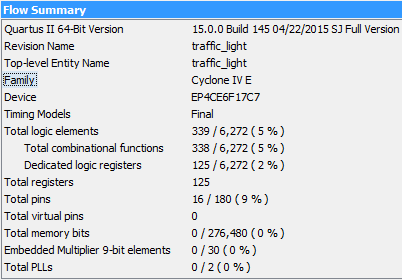
\includegraphics[width=11cm]{pic/result}
\end{center}

\section{仿真结果}
\begin{center}
	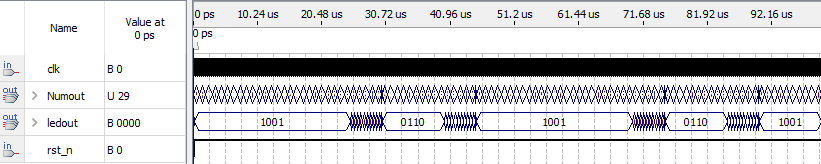
\includegraphics[width=16cm]{pic/wave}
\end{center}
局部图:
\begin{center}
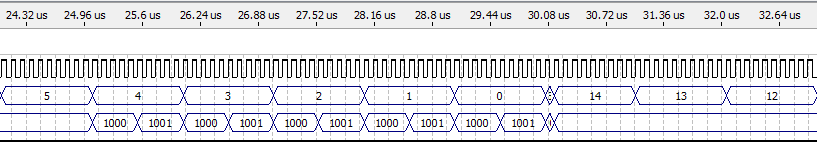
\includegraphics[width=16cm]{pic/wave2}
\end{center}

从波形图中,我们很容易看到随着时钟的输入,倒计时正常工作。当倒计时数到最后5秒时,灯输出信号不断的改变,也就是说绿灯在不断地闪烁,闪烁过程结束后,该车道的红灯亮绿灯灭,另一车道的红灯灭绿灯亮……周而复始,往复循环。

由于数码管显示模块无法仿真,在实际测试中给予展示。
\section{测试结果}
\begin{center}
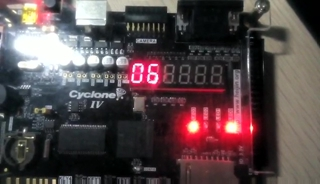
\includegraphics[width=3.8cm]{pic/test/1}
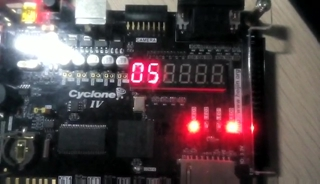
\includegraphics[width=3.8cm]{pic/test/2}
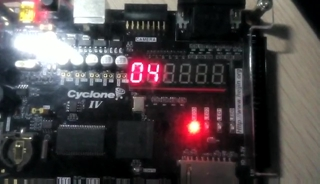
\includegraphics[width=3.8cm]{pic/test/3}
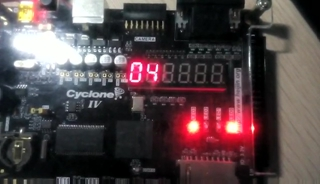
\includegraphics[width=3.8cm]{pic/test/4}

\vspace*{0.25cm}
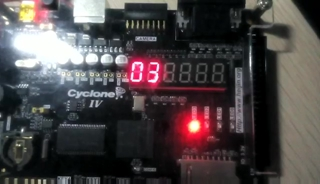
\includegraphics[width=3.8cm]{pic/test/5}
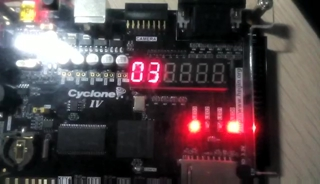
\includegraphics[width=3.8cm]{pic/test/6}
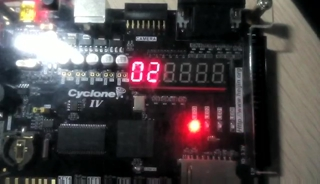
\includegraphics[width=3.8cm]{pic/test/7}
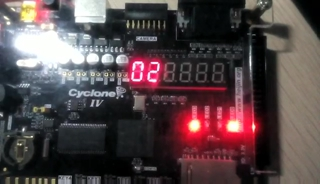
\includegraphics[width=3.8cm]{pic/test/8}

\vspace*{0.25cm}
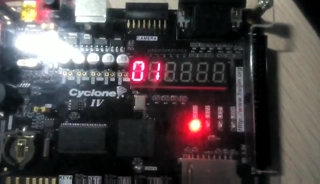
\includegraphics[width=3.8cm]{pic/test/9}
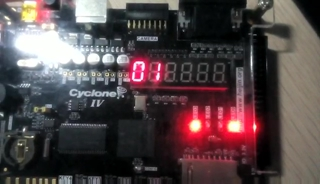
\includegraphics[width=3.8cm]{pic/test/10}
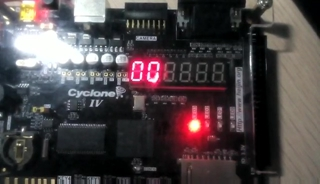
\includegraphics[width=3.8cm]{pic/test/11}
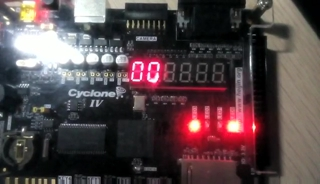
\includegraphics[width=3.8cm]{pic/test/12}

\vspace*{0.25cm}
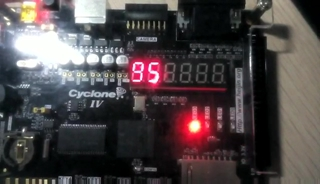
\includegraphics[width=3.8cm]{pic/test/13}
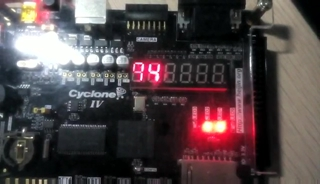
\includegraphics[width=3.8cm]{pic/test/14}
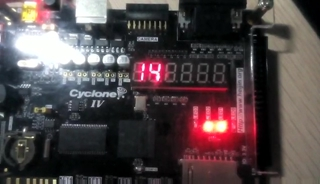
\includegraphics[width=3.8cm]{pic/test/15}
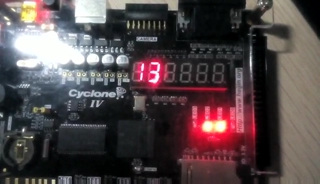
\includegraphics[width=3.8cm]{pic/test/16}
\end{center}

\section{遇到的问题}
\begin{center}
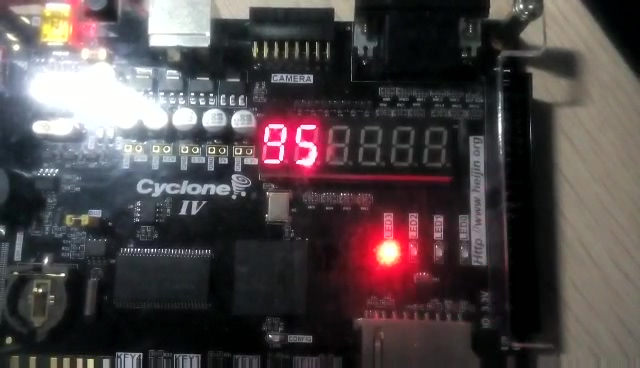
\includegraphics[width=15cm]{pic/test/17}
\vspace*{0.25cm}

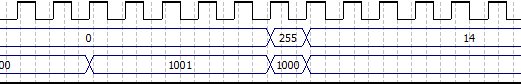
\includegraphics[width=16cm]{pic/problems}
\end{center}

在倒计时时候,X车道从Tx-1秒倒计到0秒、切换到Ty-1秒是,会有短暂的“毛刺”毛刺,如仿真波形所示。

经过初步的分析,这是由于时序状态机在进行状态判断过程中会消耗一个时钟周期所造成的。在这个时钟周期内,状态进行判断,电路来不及变化,所以产生毛刺现象。不过这个“不正常”的现象并不影响精确的倒计时的时间,因为倒计时的时间总是由输入时钟来决定,跟输出电路无关。好在这个时间持续的很短,肉眼无法明显察觉,并且不影响设计功能,所以并无大碍。

希望随着以后更深入的学习,找到这个问题的关键,并解决它。
\end{document}

